\documentclass[UTF8,a4paper,10pt]{ctexart}
\usepackage[left=2.50cm, right=2.50cm, top=2.50cm, bottom=2.50cm]{geometry}
\usepackage{times}
\usepackage{amsmath, amsfonts, amssymb} % math equations, symbols
\usepackage[english]{babel}
\usepackage{color}      % color content
\usepackage{graphicx}   % import figures
\usepackage{url}        % hyperlinks
\usepackage{bm}         % bold type for equations
\usepackage{algorithm}
\usepackage{algorithmic}
\usepackage{indentfirst}
\usepackage{subfigure}
\setlength{\parindent}{2em}

\title{\textcolor[rgb]{0,0.3,0.6}{\textbf{遗传算法+机器学习 }\\ [2ex] \begin{large} Machine\  Learning\  +\  Genetic\ Algorithm\end{large}}}
\author{Lin}
\date{\today}

\begin{document}
\maketitle
\section{\textcolor[rgb]{0,0.3,0.6}{基本框架}}
由于变异、交叉的具体实现大体类似,作曲遗传算法的核心在于适应度函数的具体实现,可以说,作曲遗传算法的好坏决定于适应度函数的好坏。但适应度函数是一个主观性特别强的内容,除去一些普适性的规律直往外,不同的人依据不同的规则和音乐认知,将给出完全不同的适应度函数,所以我们决定尝试着采用机器学习(Machine Learning)的方式实现适应度函数,通过机器学习来提取旋律中的特征,以此去除人为适应度函数的主观性。具体地说,我们将训练一个分类器(Classifier),将不同的旋律划分为好(1)与不好(0),将旋律被划分为好(1)的概率作为其适应度函数,再利用遗传算法进行作曲(图1)。
\begin{figure}[H]
\begin{center}
	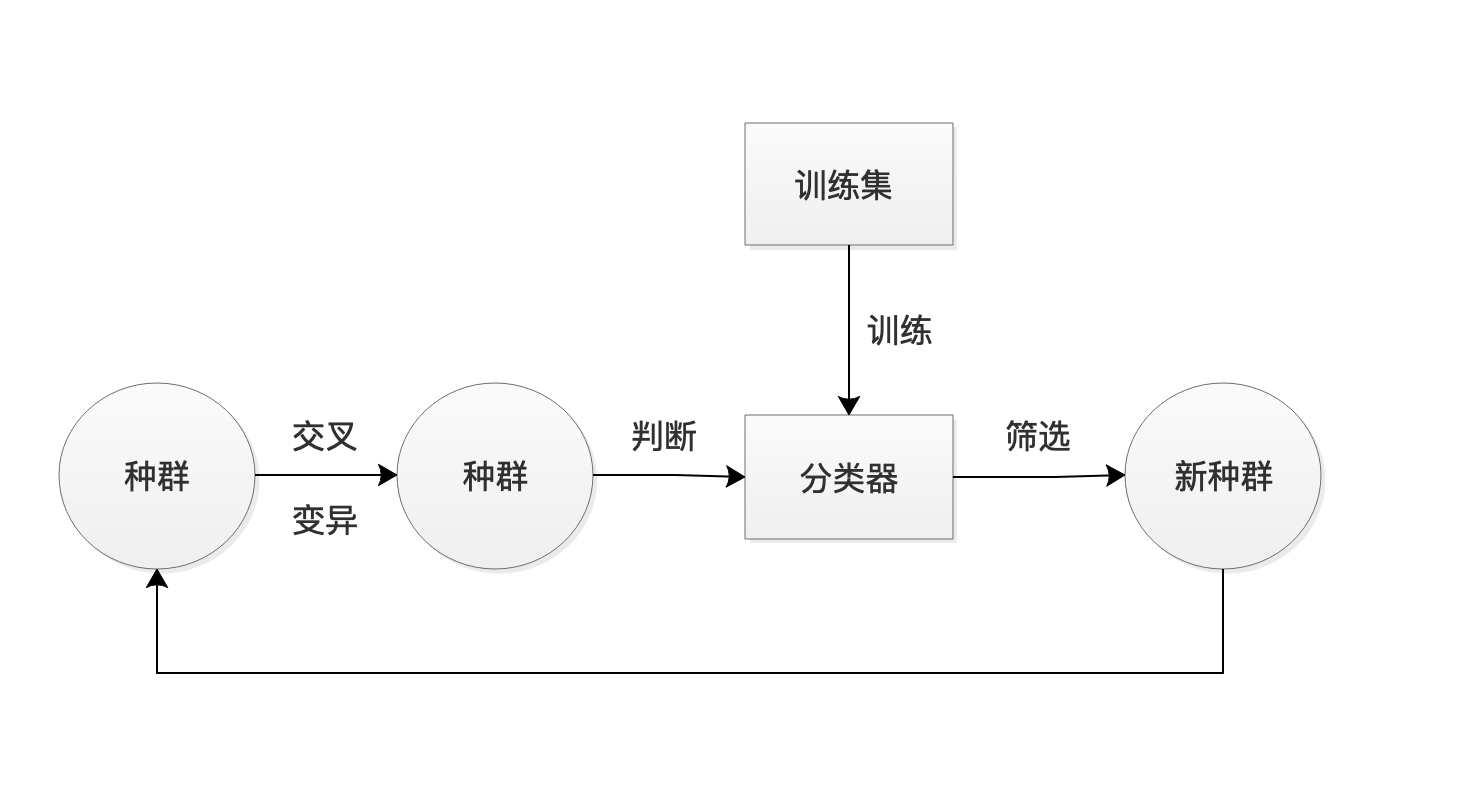
\includegraphics[width=0.7\columnwidth]{flow_chart.png}
	\caption{基本框架}
\end{center}
\end{figure}

\section{\textcolor[rgb]{0,0.3,0.6}{训练集构建}}
\subsection{MID文件解析}
相对于其他文件格式,MID文件是较为简单明了,可以明确解析的文件格式。在MID文件中,设置速度、改换音色、增减音轨都是以一个特殊的Event形式存在,特别地,增添音符则以NoteOnEvent,NoteOffEvent两个事件构成,其中NoteOnEvent可视为音符的开始,NoteOffEvent可视为音符的结束,NoteOnEvent和NoteOffEvent均具有三个参数,分别是tick,pitch,velocity,其中tick是时间量(在MID文件中,一般480ticks代表一拍),pitch代表音高(在MID文件中,中央C的pitch为60,每增减一个半音,pitch数值将增减一),velocity则代表力度。三个参数可以被分别读取,这就为我们解析MID文件提供了便利。具体来讲,Python已有现行的库对MID文件进行解析,本文使用的是PythonMIDI,MIDO,PrettyMIDI三个库,三个库均可以在GitHub上找到下载。midi解析的代码见midi\_coding.py文件,在该代码文件中,我们将MID文件转化成了Python 的Numpy二维数组,数组中的每一个值均为一个三维向量[tick,pitch,velocity],在后续的过程中,将使用该向量的形式进行学习。

\subsection{训练集的选取和构建}
由于现行的MID文件训练集的资源较少,我们寻找到了134个来自巴赫不同作品的MID文件。出于不同乐器音色不同的考虑,我们将MID文件中的每一个钢琴音轨(MID文件中ProgramChangeEvent的参数在0~7之间代表这个音轨是琴音轨)提取出,共提取出了125个音轨,这些音轨有长有短,而大多数机器学习方法要求输入的向量长度相同,于是我们在每次训练的时候,将随机地从125个音轨中抽取定长的音符片段,形成一个标记为1的训练样本,总共抽取1000个。而标记为0的训练样本则通过随机生成(我们认定随机生成的旋律一定是不好听的或好听的概率很小),将标记为1和标记为0的训练样本合并就得到全体训练集。生成训练集的代码位于代码文件model\_training.py中。


\section{\textcolor[rgb]{0,0.3,0.6}{学习器的选择和训练}}
\subsection{传统学习模型}
本文采取的传统学习模型主要有逻辑斯蒂回归(Logistic Regression,其中代表惩罚项的参数C=100),多层感知机(Multilayer Perceptrons, MLP,其中包含1000个隐藏层,每层包括100个神经元),随机森林(Random Forest,其中代表集成学习分类器个数的参数n\_estimators=100)三种模型。其中逻辑斯蒂回归的原理最为简单,采用的是线性模型和随机森林的原理则稍为复杂,以上三种学习模型的原理可以在任何一本机器学习的教材中找到,此处不再赘述。

本次使用的传统学习方法都集成于Python的sklearn库中,训练学习器的代码位于代码文件model\_t\ raining.py中,训练好的模型将直接存储在models文件夹中,分别存储为logreg.model,mlp.model,forest.model,方便使用时读取。训练时将全体训练集以3:1的比例划分为训练集和验证集,三种模型在训练集上的分类正确率均较好,但在验证集上逻辑斯蒂回归表现不佳,多层感知机和随机森林则仍旧保持着较高的正确率,某一次训练的训练集、验证集正确率(Accuracy)见表1。
\makeatletter\def\@captype{table}\makeatother
\begin{center}
\caption{不同学习模型的分类正确率表}
\begin{tabular}{c|c|c}
\hline
学习模型 & 训练集正确率 & 验证集正确率 \\ \hline
逻辑斯蒂回归 & 0.921 & 0.764 \\ \hline
多层感知机 & 0.918 &  0.926 \\ \hline
随机森林 & 1.0 & 0.995 \\ \hline
\end{tabular}
\end{center}

这点也可以简单地从不同学习模型的特性分析出。对于逻辑斯蒂回归来说,每一个音的tick,pitch,\  velocity三个性质都是一个独立的维度,对于64个音符的片段,就相当于192维的向量,而且这192个维度互相独立,互不影响,没有联系,当使用逻辑斯蒂回归进行分类时,分类器将分别考虑每一个位置上的音符,而并没有考虑音符之间的关系(即各个维度之间的关系),对旋律而言,这种考量是不科学的,旋律的好听与否,在很大程度上取决于其音间关系 (例如音程关系),所以我们可以断言逻辑斯蒂回归这种简单的几乎全线性(惩罚项$||\beta||_2^2$赋予了其一定的非线性性)的模型并不适合用于学习旋律这样维度之间存在或显性或隐性关系的样本。相反由于多层感知机在每经历一次全连接层的线性变化之后都会通过某一个阈值函数(例如RELU,或是tanh函数)对输出的结果进行一定的非线性变换,此时音间关系就有可能被学得,随机森林基于决策树方法,在集成学习的整体框架下,音间关系也是有可能被学习的。

\subsection{深度学习模型}

对于旋律特征的学习和提取而言,传统的学习模型仍然具有难以避开的问题。对于一段乐曲而言,例如它的编码是$[a_1,a_2...a_{64}]$,此时我们判断它是“好听的”,对于传统的学习模型,其每个音符的位置时固定的,也就是说,传统学习模型认为只有在$a_1$处于第0个位置,$a_2$处于第1个位置...$a_{64}$处于第63个位置的时候才是好听的,如果我们将乐曲做时间上整体平移,再在头尾适当增补某些音符(例如将编码变为$[a_0,a_1...a_{63}]$),就我们人来说应该大概率也是好听的,但此时传统学习模型训练处的分类器很有可能就认为其“难听”,也就是说,传统学习模型很难学习出旋律的这种“时间平移对称性”的特征。

据此联想到被广泛用于图像数据处理的卷积神经网络(Convolutional Neural Networks, CNN),由于图像在局部的区域内同样存在平移对称性,而卷积操作可以在一定程度上将这种特征提取出来,那么对于旋律在时间轴上的对称性,利用一维卷积操作应该也可以一定程度上在分类器中保留这种特征。

在music\_net.py文件中,使用PyTorch库搭建了一个包含多个卷积层、最大池化层和若干全连接层的小型神经网络(MusicNet),具体结构如图2。(输入向量的每一维代表一个音符,一个音符含有3个参数,于是输入的通道数为3,图中以长度为64个音符的旋律举例)
\begin{figure}[H]
\begin{center}
	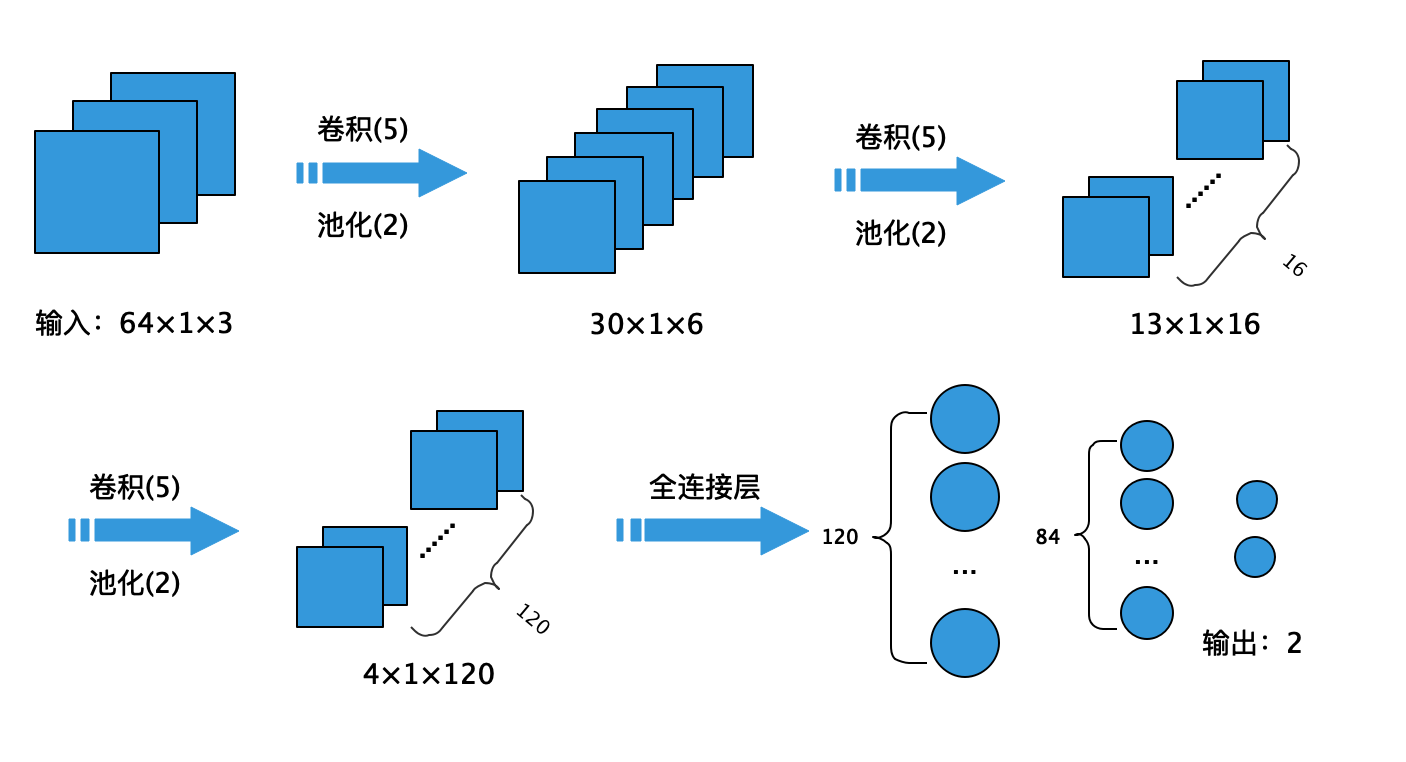
\includegraphics[width=0.7\columnwidth]{CNN_net_structure.png}
	\caption{MusicNet结构}
\end{center}
\end{figure}

该网络以交叉熵(CrossEntropy)为损失函数,采用SGD小批量随机梯度下降方法,学习率为0.001,动量参数momentum为0.9,在前述训练集下以小批量(batch\_size=50)训练50代,此时损失函数已经基本降至0,训练好的网络在训练集和验证集上的分类正确率均在0.995以上。此时将训练好的网络参数存储至models文件夹下的music\_net.tar,方便使用时读取。



\section{\textcolor[rgb]{0,0.3,0.6}{基于机器学习的遗传算法作曲}}
遗传算法的整体框架和前述的人工适应度函数所用框架大致相同,由于旋律的具体表现形式不同(此处将音符的时值和力度特性以另外两个维度的形式体现,所以同样长度为64的旋律,人工适应度函数的编码是长度为64的向量,而此处的编码为64行3列的矩阵),所以对各个部分略作修改,具体实现已集成于main.py文件中,变异部分(见Population类的mutation函数)包含单个音符的变异、整体移调、逆行和倒影,并设置变异率为0.1,选择部分则使用遗传算法常用的轮盘赌算法(见Population类的selection函数),计算适应度时则直接用特定的学习器对输入的音符矩阵进行概率预测(predict\_proba,见Individual类的cal\_fitness函数),在实验时规定种群大小为30,迭代代数为1000代,1000代之后选取种群中最好的个体,用集成于midi\_coding.py文件中的reconversion函数将其转化为midi文件输出。

实验中在每一代提取其个体适应度的平均值,作图如图3-图6所示。

\begin{figure}[H]
\begin{minipage}[t]{0.5\linewidth}
\centering
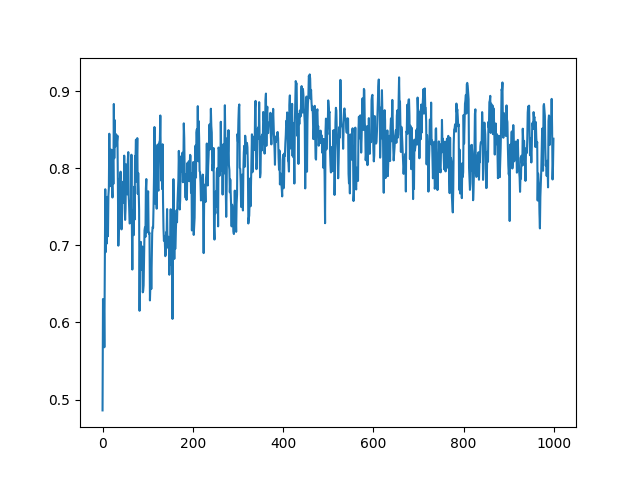
\includegraphics[width=3in]{output_logreg.png}
\caption{Logistic Regression}
\label{fig:side:a}
\end{minipage}%
\begin{minipage}[t]{0.5\linewidth}
\centering
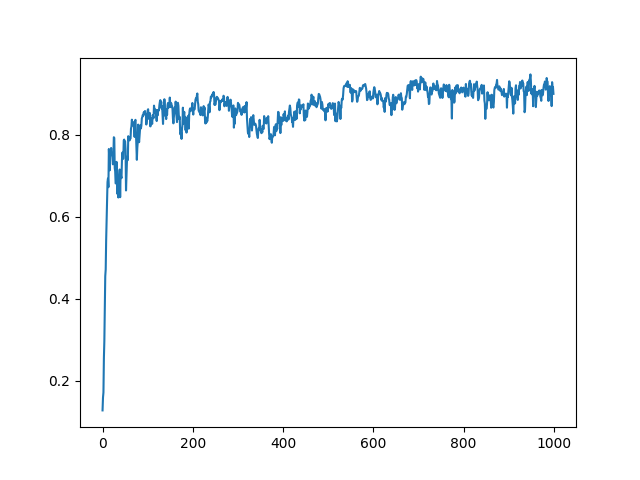
\includegraphics[width=3in]{output_mlp.png}
\caption{MLP}
\label{fig:side:b}
\end{minipage}
\end{figure}

\begin{figure}[H]
\begin{minipage}[t]{0.5\linewidth}
\centering
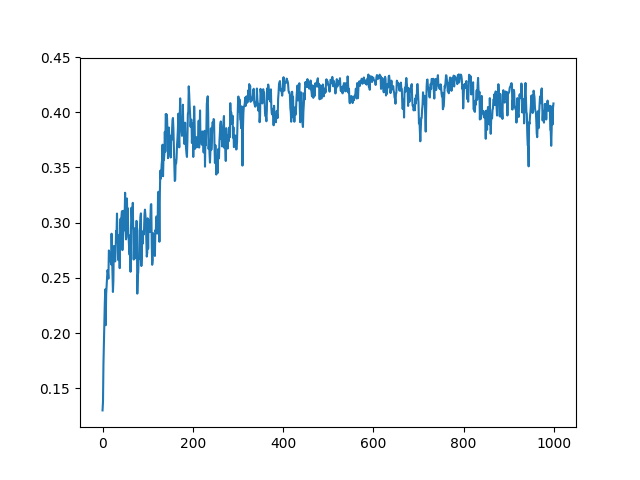
\includegraphics[width=3in]{output_forest.png}
\caption{Random Forest}
\label{fig:side:a}
\end{minipage}%
\begin{minipage}[t]{0.5\linewidth}
\centering
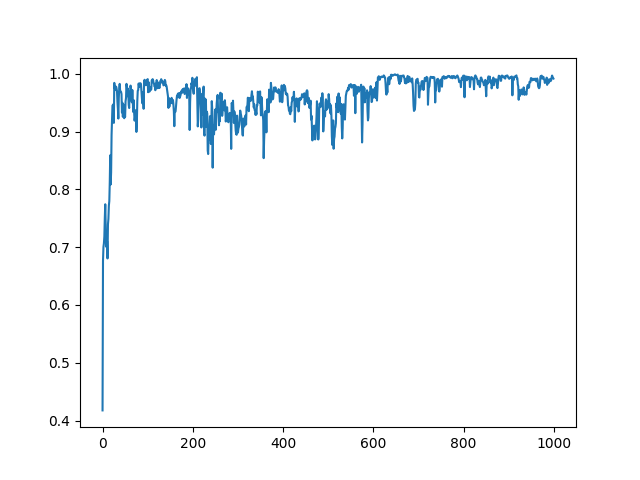
\includegraphics[width=3in]{output_cnn.png}
\caption{CNN}
\label{fig:side:b}
\end{minipage}
\end{figure}

从这四幅图中可以发现一些有意思的现象。在迭代1000代之后,四种学习模型都已经达到了一个稳定值,由于变异的存在,以稳定值为中心上下波动。对于逻辑斯蒂回归,它的迭代起点相当高(接近0.5),这就说明在种群初始化时,我们随机生成的音符片段被认为是“好听的”概率在0.5以上,这显然是荒谬的,并且其在后续迭代的过程中上下波动相当剧烈,这就说明在小范围变异(变异率为0.1,这是一个相对较小的值)的作用下其种群的分类概率可以发生显著波动,这显然也不符合旋律片段将在遗传算法作用下最终收敛的特性。MLP和CNN由于原理大体类似,在遗传算法作用下显示出了相似的图像,在迭代后期波动较小,有收敛至1(说明其可以产生一个分类器认为是“绝对好听”的旋律)的趋势,CNN已经接近收敛于1。随机森林则在迭代1000次以后,最高的平均适应度仍然不及0.45,换言之,在迭代1000次后仍然不能产生一个令随机森林分类器“满意”的个体,这说明随机森林对“好”的要求较为严苛,限制较多,随机森林的学习模型很有可能存在“过拟合”的风险。

在经过试验之后,产生的乐曲片段都已经转化成MIDI文件存储在output\_melody文件夹中,其五线谱如图7-图10所示。
\begin{figure}[H]
\begin{center}
	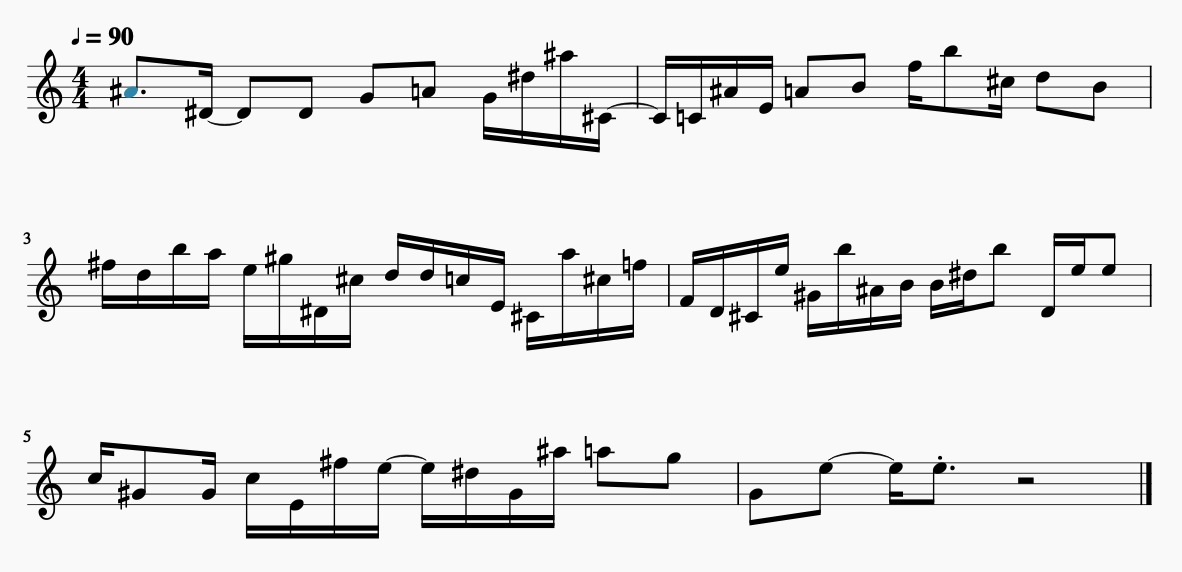
\includegraphics[width=1.0\columnwidth]{output_logreg_melody.png}
	\caption{Logistic Regression}
\end{center}
\end{figure}

\begin{figure}[H]
\begin{center}
	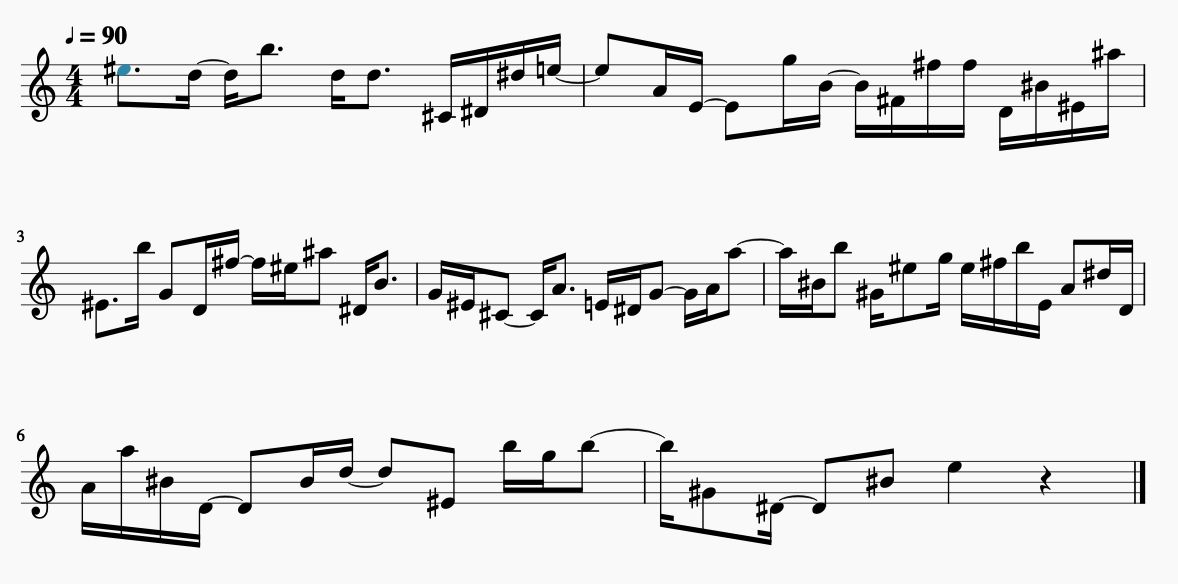
\includegraphics[width=1.0\columnwidth]{output_mlp_melody.png}
	\caption{MLP}
\end{center}
\end{figure}

\begin{figure}[H]
\begin{center}
	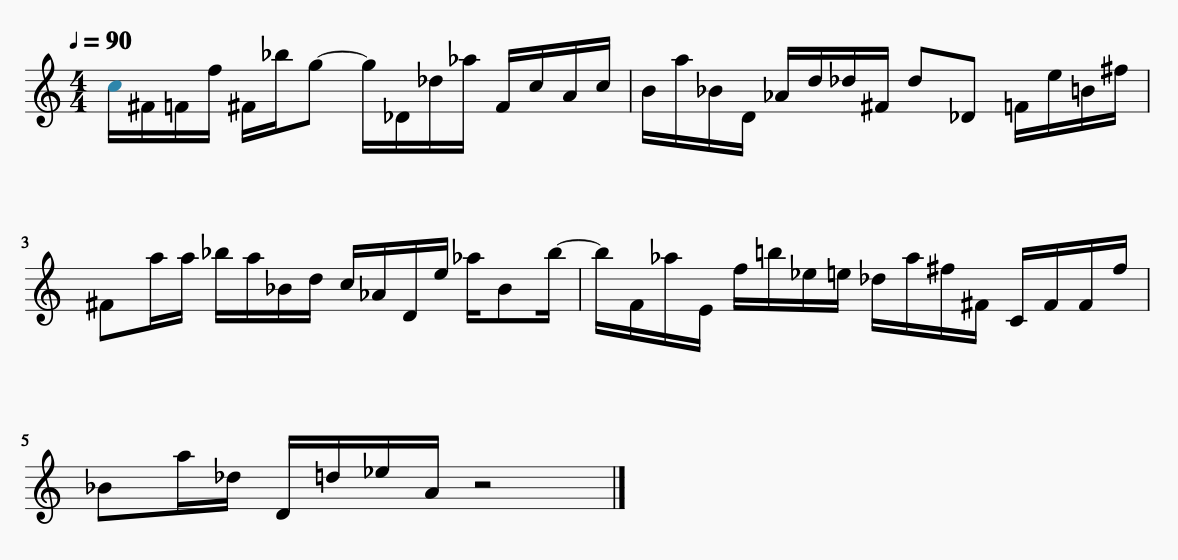
\includegraphics[width=1.0\columnwidth]{output_forest_melody.png}
	\caption{Random Forest}
\end{center}
\end{figure}

\begin{figure}[H]
\begin{center}
	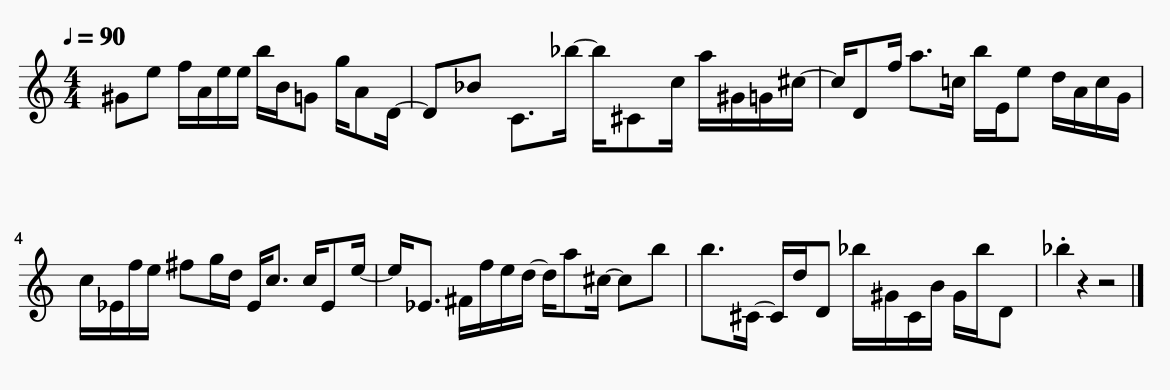
\includegraphics[width=1.0\columnwidth]{output_cnn_melody.png}
	\caption{CNN}
\end{center}
\end{figure}

可以说,这四段旋律都不能算好听,甚至有些刺耳 ,经过对这几段旋律的简单,我们认为其不好听的原因可能有以下几个:
\begin{itemize}
	\item 节奏型乱。这点可以追溯到我们训练集构建的部分,在训练集构建的过程中,我们所选取的134个MID文件具有不同的节奏型和节拍,并且我们在构建训练集的时候是随机截取的定长音符的音轨片段,而不是以小节为片段进行截取,而节奏型与小节的划分具有密切联系,这使得在我们的训练集中,时值(tick)这一维度的数据是近似随机的,在用学习模型进行特征提取的时候提取出的特征也是近似随机的,最终产生旋律的节奏型效果并不好。这个问题的解决方案是按照完整乐句截取训练集,但对于MID文件格式,由于其没有记录节拍、小节划分的数据,所以分割乐句的任务具有难度,目前除了手动筛选以外没有其他的解决方案,所以节奏型上很难再进行改良。
	\item 音程跳跃大,听起来不稳定。我们对某次实验中四种学习器输出的旋律编码进行了差分,取绝对值之后对其进行了统计,绘制直方图如图11-14所示(横轴代表半音数,纵轴代表其出现次数)。我们可以较为明显地看到,逻辑斯蒂回归的各个半音音程出现的较为平均,大跳跃(指半音数大于等于12,即8度以上)音程也占比比较高,这和前面分析的逻辑斯蒂回归并不能处理音间关系的推论是符合的。对于剩下的三种学习模型,大音程占比变少,但仍然普遍存在,占比最高的音程普遍位于5~8左右,可能对应纯四度(对应5个半音)、纯五度音程(对应7个半音 ),但不可避免地产生增四度(对应6个半音)、减五度(对应6个半音)这种并不使人愉悦的音程关系。而使人产生稳定感的大二度、小二度或是重音虽有出现,频率不大,这使得悦耳旋律中经常出现的连续上下行在输出旋律中很少出现,也就是说,在输出的旋律之中存在“忽上忽下”的跳跃情形,各个音之间较为零散,构不成完整的乐句,更不要提“旋律复现”。对于这一点,我们能做的改良仍然是有限的,由于机器学习算法的复杂性,我们不能很直观地得知机器到底从训练集中提取到了什么特征,我们也无从知晓一个具体的学习器是如何处理对应的音间关系的,无从知晓分类器是仅仅处理相邻两个维度的关系,还是考虑到了更高阶的维度联系。我们能够想到的改良方案是将输入向量进行音高差分之后与原来的编码向量合并,将相邻两个音的音间关系作为独立维度进行训练学习,但尝试的效果并不佳,可能需要考虑更高阶的音程关系。
\begin{figure}[H]
\begin{minipage}[t]{0.5\linewidth}
\centering
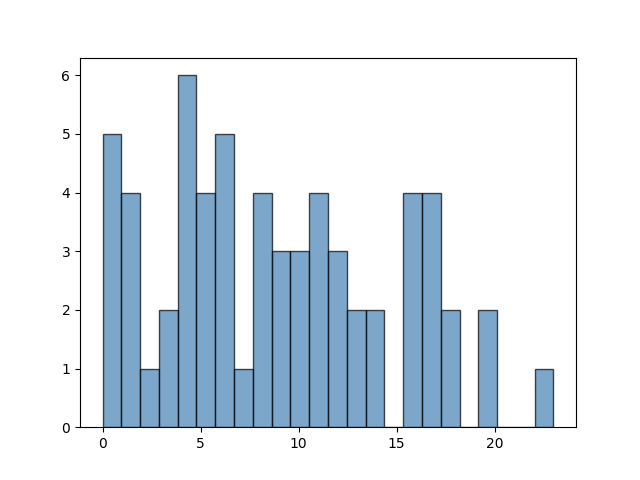
\includegraphics[width=3in]{output_logreg_hist.png}
\caption{Logistic Regression}
\label{fig:side:a}
\end{minipage}%
\begin{minipage}[t]{0.5\linewidth}
\centering
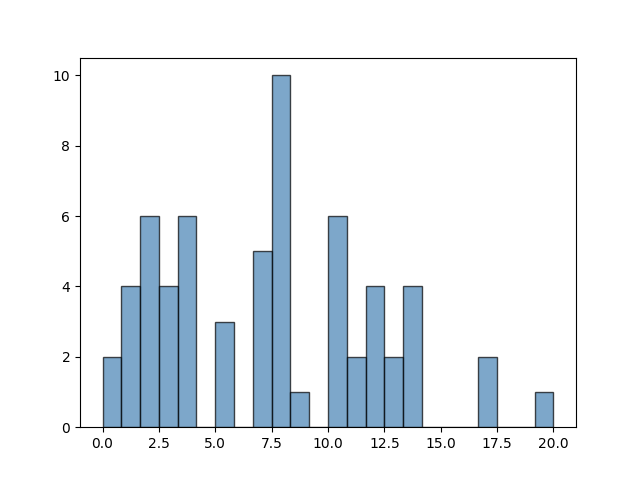
\includegraphics[width=3in]{output_mlp_hist.png}
\caption{MLP}
\label{fig:side:b}
\end{minipage}
\end{figure}

\begin{figure}[H]
\begin{minipage}[t]{0.5\linewidth}
\centering
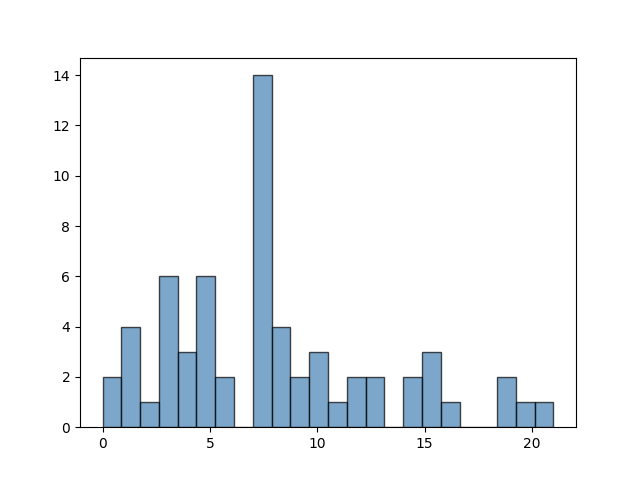
\includegraphics[width=3in]{output_forest_hist.png}
\caption{Random Forest}
\label{fig:side:a}
\end{minipage}%
\begin{minipage}[t]{0.5\linewidth}
\centering
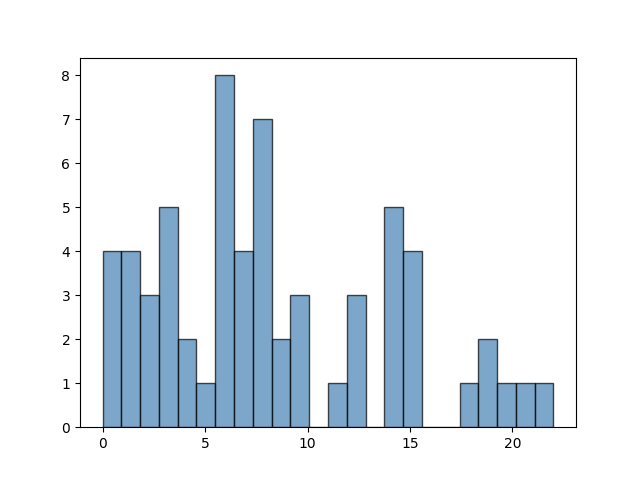
\includegraphics[width=3in]{output_cnn_hist.png}
\caption{CNN}
\label{fig:side:b}
\end{minipage}
\end{figure}
\item 不在调上的音占比高。考虑到训练集的作品C大调占了多数,从C大调的角度去分析,在某一次实验中  四种方法不在调上的音符占比如表2。
\makeatletter\def\@captype{table}\makeatother
\begin{center}
\caption{不同学习模型的输出旋律调性分析}
\begin{tabular}{c|c|c|c}
\hline
学习模型 & 音符总数 & 在调式中的音符个数 & 调性音符占比 \\ \hline
逻辑斯蒂回归 & 64 & 40 & 62.5\% \\ \hline
多层感知机 & 64 &  34 & 53.1\% \\ \hline
随机森林 & 64 & 38 & 59.4\%\\ \hline
卷积神经网络 & 64 & 47 & 73.4\% \\ \hline
\end{tabular}
\end{center}

调性音符占比呈现出了较强的随机性,旋律并没有对调性音符产生强烈的偏好,这可能也与我们选取训练集中含有部分非大调的乐曲有关,也有可能是机器学习算法本身的缺陷使旋律的调性特征没有被习得。我们同样可以对其中出现的音高做统计,绘制直方图如图15-19,可以看到,算法本身并没有对某些音具有明显的偏好,统计呈现较强的均匀性和随机性。关于这点,我们曾经尝试在在生成种群个体时仅仅使用C大调上的音,变异也限制于C大调,这时候如果使用相同的分类器进行迭代,迭代1000代之后种群的平均适应度仍然很难达到0.7,也就是说如果将音局限于C大调,分类器将不认为它是一段好听的旋律。值得一提的是,如果将个体限制在五声音阶(CDEGA)上,所有音之间的音程关系都较好,此时就算随机生成的旋律也非常悦耳,但分类器仍然不认为其是好听的。

\begin{figure}[H]
\begin{minipage}[t]{0.5\linewidth}
\centering
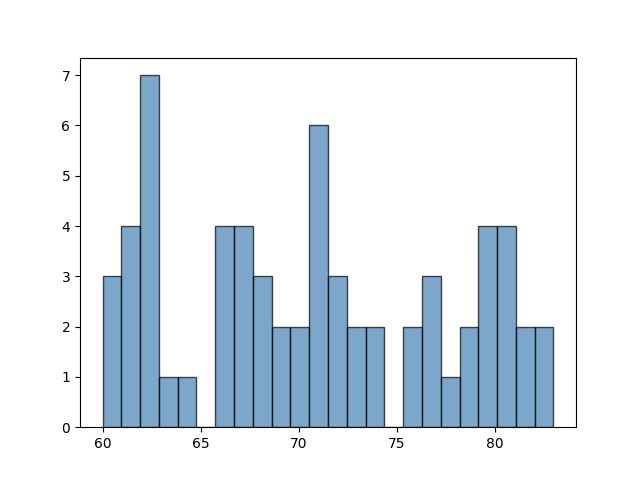
\includegraphics[width=3in]{output_logreg_hist_1.png}
\caption{Logistic Regression}
\label{fig:side:a}
\end{minipage}%
\begin{minipage}[t]{0.5\linewidth}
\centering
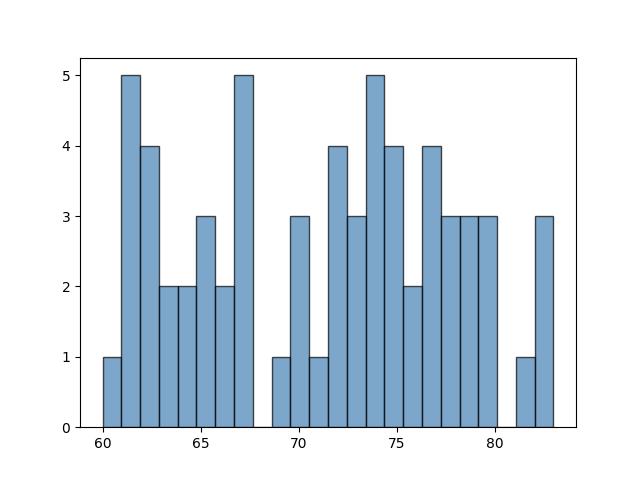
\includegraphics[width=3in]{output_mlp_hist_1.png}
\caption{MLP}
\label{fig:side:b}
\end{minipage}
\end{figure}

\begin{figure}[H]
\begin{minipage}[t]{0.5\linewidth}
\centering
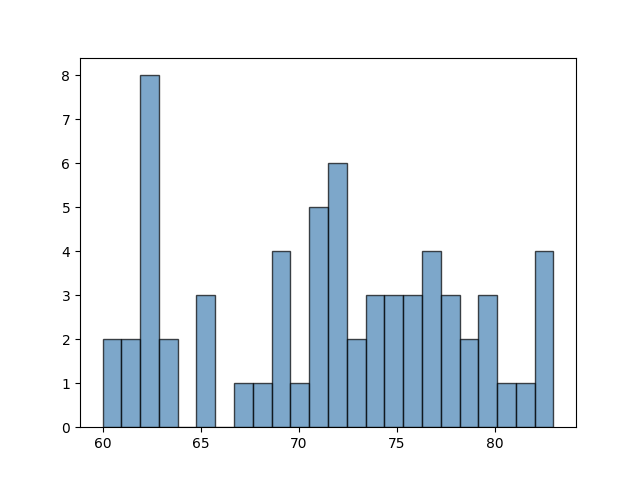
\includegraphics[width=3in]{output_forest_hist_1.png}
\caption{Random Forest}
\label{fig:side:a}
\end{minipage}%
\begin{minipage}[t]{0.5\linewidth}
\centering
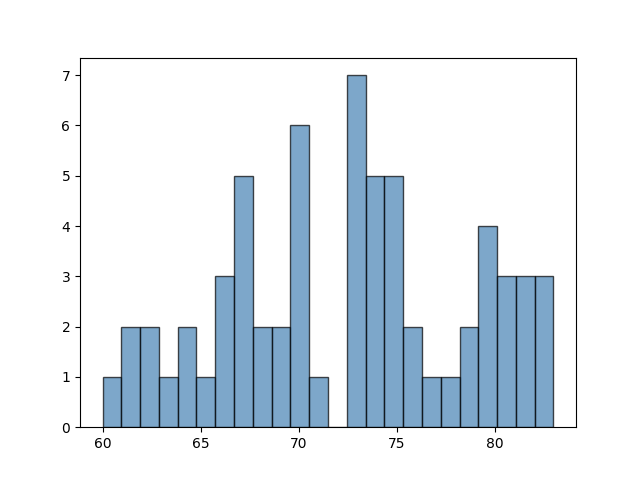
\includegraphics[width=3in]{output_cnn_hist_1.png}
\caption{CNN}
\label{fig:side:b}
\end{minipage}
\end{figure}
\end{itemize}

\section{\textcolor[rgb]{0,0.3,0.6}{总结}}

本模块旨在通过机器学习算法提取悦耳旋律的特征,构建分类器作为适应度函数的判据来排除人工适应度函数的主观性,或去发掘一些人无法感知的音乐特征。最终给出的旋律并不理想,这可能与训练集的选取,分类器的构建相关,由于机器学习算法的“黑箱特性”,我们无法直观地理解机器在分类时的判断依据,后续改良只能通过调整参数,改变训练集来逐步摸索实现。在后续的实验中,我们尝试着手动筛选了20个节奏型相近、同属于C大调、音乐风格相近的完整乐句,但由于20个样本的训练集过小,训练过程的随机性较大,产生的结果也并不理想。要使机器学习适应度函数真正能够写出悦耳动听的旋律还需要后续的改良。
\end{document}